

\tikzset{every picture/.style={line width=0.75pt}} %set default line width to 0.75pt        

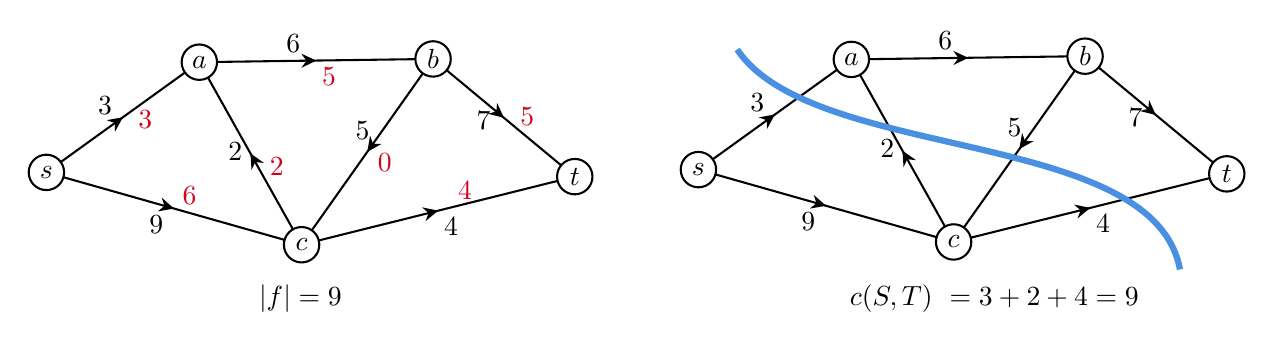
\begin{tikzpicture}[x=0.5pt,y=0.5pt,yscale=-1,xscale=1]
%uncomment if require: \path (0,225); %set diagram left start at 0, and has height of 225

%Straight Lines [id:da9082688563234774] 
\draw    (236.22,169.11) -- (331.22,34.84) ;
\draw [shift={(283.72,101.98)}, rotate = 305.28] [fill={rgb, 255:red, 0; green, 0; blue, 0 }  ][line width=0.08]  [draw opacity=0] (10.72,-5.15) -- (0,0) -- (10.72,5.15) -- (7.12,0) -- cycle    ;
%Straight Lines [id:da4024226568643945] 
\draw    (162.31,37.18) -- (236.22,169.11) ;
\draw [shift={(199.27,103.14)}, rotate = 60.74] [fill={rgb, 255:red, 0; green, 0; blue, 0 }  ][line width=0.08]  [draw opacity=0] (10.72,-5.15) -- (0,0) -- (10.72,5.15) -- (7.12,0) -- cycle    ;
%Straight Lines [id:da7912195585462996] 
\draw    (51.79,116.83) -- (236.22,169.11) ;
\draw [shift={(144.01,142.97)}, rotate = 195.83] [fill={rgb, 255:red, 0; green, 0; blue, 0 }  ][line width=0.08]  [draw opacity=0] (10.72,-5.15) -- (0,0) -- (10.72,5.15) -- (7.12,0) -- cycle    ;
%Straight Lines [id:da213272602991051] 
\draw    (433.62,119.9) -- (236.22,169.11) ;
\draw [shift={(334.92,144.5)}, rotate = 166] [fill={rgb, 255:red, 0; green, 0; blue, 0 }  ][line width=0.08]  [draw opacity=0] (10.72,-5.15) -- (0,0) -- (10.72,5.15) -- (7.12,0) -- cycle    ;
%Straight Lines [id:da8511890231681417] 
\draw    (51.79,116.83) -- (162.31,37.18) ;
\draw [shift={(107.05,77)}, rotate = 144.22] [fill={rgb, 255:red, 0; green, 0; blue, 0 }  ][line width=0.08]  [draw opacity=0] (10.72,-5.15) -- (0,0) -- (10.72,5.15) -- (7.12,0) -- cycle    ;
%Straight Lines [id:da36886265290248843] 
\draw    (331.22,34.84) -- (433.62,119.9) ;
\draw [shift={(382.42,77.37)}, rotate = 219.71] [fill={rgb, 255:red, 0; green, 0; blue, 0 }  ][line width=0.08]  [draw opacity=0] (10.72,-5.15) -- (0,0) -- (10.72,5.15) -- (7.12,0) -- cycle    ;
%Straight Lines [id:da5107251195982034] 
\draw    (162.31,37.18) -- (331.22,34.84) ;
\draw [shift={(246.76,36.01)}, rotate = 179.21] [fill={rgb, 255:red, 0; green, 0; blue, 0 }  ][line width=0.08]  [draw opacity=0] (10.72,-5.15) -- (0,0) -- (10.72,5.15) -- (7.12,0) -- cycle    ;
%Shape: Ellipse [id:dp4938989418762101] 
\draw  [fill={rgb, 255:red, 255; green, 255; blue, 255 }  ,fill opacity=1 ] (39,116.83) .. controls (39,109.77) and (44.73,104.04) .. (51.79,104.04) .. controls (58.86,104.04) and (64.58,109.77) .. (64.58,116.83) .. controls (64.58,123.9) and (58.86,129.62) .. (51.79,129.62) .. controls (44.73,129.62) and (39,123.9) .. (39,116.83) -- cycle ;
%Shape: Ellipse [id:dp7740460741911303] 
\draw  [fill={rgb, 255:red, 255; green, 255; blue, 255 }  ,fill opacity=1 ] (149.52,37.18) .. controls (149.52,30.11) and (155.25,24.39) .. (162.31,24.39) .. controls (169.38,24.39) and (175.1,30.11) .. (175.1,37.18) .. controls (175.1,44.24) and (169.38,49.97) .. (162.31,49.97) .. controls (155.25,49.97) and (149.52,44.24) .. (149.52,37.18) -- cycle ;
%Shape: Ellipse [id:dp7874695049462108] 
\draw  [fill={rgb, 255:red, 255; green, 255; blue, 255 }  ,fill opacity=1 ] (318.43,34.84) .. controls (318.43,27.78) and (324.15,22.05) .. (331.22,22.05) .. controls (338.28,22.05) and (344.01,27.78) .. (344.01,34.84) .. controls (344.01,41.9) and (338.28,47.63) .. (331.22,47.63) .. controls (324.15,47.63) and (318.43,41.9) .. (318.43,34.84) -- cycle ;
%Shape: Ellipse [id:dp5976477726175576] 
\draw  [fill={rgb, 255:red, 255; green, 255; blue, 255 }  ,fill opacity=1 ] (223.43,169.11) .. controls (223.43,162.05) and (229.15,156.32) .. (236.22,156.32) .. controls (243.28,156.32) and (249.01,162.05) .. (249.01,169.11) .. controls (249.01,176.18) and (243.28,181.9) .. (236.22,181.9) .. controls (229.15,181.9) and (223.43,176.18) .. (223.43,169.11) -- cycle ;
%Shape: Ellipse [id:dp8582649844509285] 
\draw  [fill={rgb, 255:red, 255; green, 255; blue, 255 }  ,fill opacity=1 ] (420.83,119.9) .. controls (420.83,112.83) and (426.56,107.11) .. (433.62,107.11) .. controls (440.69,107.11) and (446.41,112.83) .. (446.41,119.9) .. controls (446.41,126.96) and (440.69,132.69) .. (433.62,132.69) .. controls (426.56,132.69) and (420.83,126.96) .. (420.83,119.9) -- cycle ;
%Straight Lines [id:da7220126124754225] 
\draw    (707.43,167.11) -- (802.42,32.84) ;
\draw [shift={(754.92,99.98)}, rotate = 305.28] [fill={rgb, 255:red, 0; green, 0; blue, 0 }  ][line width=0.08]  [draw opacity=0] (10.72,-5.15) -- (0,0) -- (10.72,5.15) -- (7.12,0) -- cycle    ;
%Straight Lines [id:da8450888320434884] 
\draw    (633.52,35.18) -- (707.43,167.11) ;
\draw [shift={(670.47,101.14)}, rotate = 60.74] [fill={rgb, 255:red, 0; green, 0; blue, 0 }  ][line width=0.08]  [draw opacity=0] (10.72,-5.15) -- (0,0) -- (10.72,5.15) -- (7.12,0) -- cycle    ;
%Straight Lines [id:da28397437899635924] 
\draw    (523,114.83) -- (707.43,167.11) ;
\draw [shift={(615.21,140.97)}, rotate = 195.83] [fill={rgb, 255:red, 0; green, 0; blue, 0 }  ][line width=0.08]  [draw opacity=0] (10.72,-5.15) -- (0,0) -- (10.72,5.15) -- (7.12,0) -- cycle    ;
%Straight Lines [id:da37734529713635245] 
\draw    (904.83,117.9) -- (707.43,167.11) ;
\draw [shift={(806.13,142.5)}, rotate = 166] [fill={rgb, 255:red, 0; green, 0; blue, 0 }  ][line width=0.08]  [draw opacity=0] (10.72,-5.15) -- (0,0) -- (10.72,5.15) -- (7.12,0) -- cycle    ;
%Straight Lines [id:da0928727354789407] 
\draw    (523,114.83) -- (633.52,35.18) ;
\draw [shift={(578.26,75)}, rotate = 144.22] [fill={rgb, 255:red, 0; green, 0; blue, 0 }  ][line width=0.08]  [draw opacity=0] (10.72,-5.15) -- (0,0) -- (10.72,5.15) -- (7.12,0) -- cycle    ;
%Straight Lines [id:da48901200769836506] 
\draw    (802.42,32.84) -- (904.83,117.9) ;
\draw [shift={(853.63,75.37)}, rotate = 219.71] [fill={rgb, 255:red, 0; green, 0; blue, 0 }  ][line width=0.08]  [draw opacity=0] (10.72,-5.15) -- (0,0) -- (10.72,5.15) -- (7.12,0) -- cycle    ;
%Straight Lines [id:da42638454833244943] 
\draw    (633.52,35.18) -- (802.42,32.84) ;
\draw [shift={(717.97,34.01)}, rotate = 179.21] [fill={rgb, 255:red, 0; green, 0; blue, 0 }  ][line width=0.08]  [draw opacity=0] (10.72,-5.15) -- (0,0) -- (10.72,5.15) -- (7.12,0) -- cycle    ;
%Shape: Ellipse [id:dp8396933555638321] 
\draw  [fill={rgb, 255:red, 255; green, 255; blue, 255 }  ,fill opacity=1 ] (510.21,114.83) .. controls (510.21,107.77) and (515.94,102.04) .. (523,102.04) .. controls (530.06,102.04) and (535.79,107.77) .. (535.79,114.83) .. controls (535.79,121.9) and (530.06,127.62) .. (523,127.62) .. controls (515.94,127.62) and (510.21,121.9) .. (510.21,114.83) -- cycle ;
%Shape: Ellipse [id:dp26514516487162165] 
\draw  [fill={rgb, 255:red, 255; green, 255; blue, 255 }  ,fill opacity=1 ] (620.73,35.18) .. controls (620.73,28.11) and (626.46,22.39) .. (633.52,22.39) .. controls (640.58,22.39) and (646.31,28.11) .. (646.31,35.18) .. controls (646.31,42.24) and (640.58,47.97) .. (633.52,47.97) .. controls (626.46,47.97) and (620.73,42.24) .. (620.73,35.18) -- cycle ;
%Shape: Ellipse [id:dp08880583589515356] 
\draw  [fill={rgb, 255:red, 255; green, 255; blue, 255 }  ,fill opacity=1 ] (789.63,32.84) .. controls (789.63,25.78) and (795.36,20.05) .. (802.42,20.05) .. controls (809.49,20.05) and (815.21,25.78) .. (815.21,32.84) .. controls (815.21,39.9) and (809.49,45.63) .. (802.42,45.63) .. controls (795.36,45.63) and (789.63,39.9) .. (789.63,32.84) -- cycle ;
%Shape: Ellipse [id:dp5357688919708571] 
\draw  [fill={rgb, 255:red, 255; green, 255; blue, 255 }  ,fill opacity=1 ] (694.64,167.11) .. controls (694.64,160.05) and (700.36,154.32) .. (707.43,154.32) .. controls (714.49,154.32) and (720.22,160.05) .. (720.22,167.11) .. controls (720.22,174.18) and (714.49,179.9) .. (707.43,179.9) .. controls (700.36,179.9) and (694.64,174.18) .. (694.64,167.11) -- cycle ;
%Shape: Ellipse [id:dp8198953137865064] 
\draw  [fill={rgb, 255:red, 255; green, 255; blue, 255 }  ,fill opacity=1 ] (892.04,117.9) .. controls (892.04,110.83) and (897.77,105.11) .. (904.83,105.11) .. controls (911.89,105.11) and (917.62,110.83) .. (917.62,117.9) .. controls (917.62,124.96) and (911.89,130.69) .. (904.83,130.69) .. controls (897.77,130.69) and (892.04,124.96) .. (892.04,117.9) -- cycle ;
%Curve Lines [id:da631287332539116] 
\draw [color={rgb, 255:red, 74; green, 144; blue, 226 }  ,draw opacity=1 ][line width=2.25]    (551,28) .. controls (606,110) and (852,84) .. (871,187) ;

% Text Node
\draw (51.79,116.83) node   [align=left] {$\displaystyle s$};
% Text Node
\draw (162.31,37.18) node   [align=left] {$\displaystyle a$};
% Text Node
\draw (331.22,34.84) node   [align=left] {$\displaystyle b$};
% Text Node
\draw (236.22,169.11) node   [align=left] {$\displaystyle c$};
% Text Node
\draw (433.62,119.9) node   [align=left] {$\displaystyle t$};
% Text Node
\draw (124,146) node [anchor=north west][inner sep=0.75pt]   [align=left] {$\displaystyle 9$};
% Text Node
\draw (273,78) node [anchor=north west][inner sep=0.75pt]   [align=left] {$\displaystyle 5$};
% Text Node
\draw (181,93) node [anchor=north west][inner sep=0.75pt]   [align=left] {$\displaystyle 2$};
% Text Node
\draw (87,60) node [anchor=north west][inner sep=0.75pt]   [align=left] {$\displaystyle 3$};
% Text Node
\draw (336.92,147.5) node [anchor=north west][inner sep=0.75pt]   [align=left] {$\displaystyle 4$};
% Text Node
\draw (360.42,70.37) node [anchor=north west][inner sep=0.75pt]   [align=left] {$\displaystyle 7$};
% Text Node
\draw (223,15) node [anchor=north west][inner sep=0.75pt]   [align=left] {$\displaystyle 6$};
% Text Node
\draw (148,125) node [anchor=north west][inner sep=0.75pt]   [align=left] {$\displaystyle \textcolor[rgb]{0.82,0.01,0.11}{6}$};
% Text Node
\draw (211,104) node [anchor=north west][inner sep=0.75pt]   [align=left] {$\displaystyle \textcolor[rgb]{0.82,0.01,0.11}{2}$};
% Text Node
\draw (347,121) node [anchor=north west][inner sep=0.75pt]   [align=left] {$\displaystyle \textcolor[rgb]{0.82,0.01,0.11}{4}$};
% Text Node
\draw (116,70) node [anchor=north west][inner sep=0.75pt]   [align=left] {$\displaystyle \textcolor[rgb]{0.82,0.01,0.11}{3}$};
% Text Node
\draw (248.76,39.01) node [anchor=north west][inner sep=0.75pt]   [align=left] {$\displaystyle \textcolor[rgb]{0.82,0.01,0.11}{5}$};
% Text Node
\draw (289,101) node [anchor=north west][inner sep=0.75pt]   [align=left] {$\displaystyle \textcolor[rgb]{0.82,0.01,0.11}{0}$};
% Text Node
\draw (392,68) node [anchor=north west][inner sep=0.75pt]   [align=left] {$\displaystyle \textcolor[rgb]{0.82,0.01,0.11}{5}$};
% Text Node
\draw (523,114.83) node   [align=left] {$\displaystyle s$};
% Text Node
\draw (633.52,35.18) node   [align=left] {$\displaystyle a$};
% Text Node
\draw (802.42,32.84) node   [align=left] {$\displaystyle b$};
% Text Node
\draw (707.43,167.11) node   [align=left] {$\displaystyle c$};
% Text Node
\draw (904.83,117.9) node   [align=left] {$\displaystyle t$};
% Text Node
\draw (595.21,144) node [anchor=north west][inner sep=0.75pt]   [align=left] {$\displaystyle 9$};
% Text Node
\draw (744.21,76) node [anchor=north west][inner sep=0.75pt]   [align=left] {$\displaystyle 5$};
% Text Node
\draw (652.21,91) node [anchor=north west][inner sep=0.75pt]   [align=left] {$\displaystyle 2$};
% Text Node
\draw (558.21,58) node [anchor=north west][inner sep=0.75pt]   [align=left] {$\displaystyle 3$};
% Text Node
\draw (808.13,145.5) node [anchor=north west][inner sep=0.75pt]   [align=left] {$\displaystyle 4$};
% Text Node
\draw (831.63,68.37) node [anchor=north west][inner sep=0.75pt]   [align=left] {$\displaystyle 7$};
% Text Node
\draw (694.21,13) node [anchor=north west][inner sep=0.75pt]   [align=left] {$\displaystyle 6$};
% Text Node
\draw (630.21,196) node [anchor=north west][inner sep=0.75pt]   [align=left] {$\displaystyle c( S,T) \ =3+2+4=9$};
% Text Node
\draw (203.21,196) node [anchor=north west][inner sep=0.75pt]   [align=left] {$\displaystyle |f|=9$};


\end{tikzpicture}

